\documentclass[11pt]{article}

% Language setting
\usepackage[turkish]{babel}
\usepackage{pythonhighlight}

\usepackage[a4paper,top=2cm,bottom=2cm,left=2cm,right=2cm,marginparwidth=2cm]{geometry}

% Useful packages
\usepackage{amsmath}
\usepackage{graphicx}
\usepackage[colorlinks=true, allcolors=blue]{hyperref}
\usepackage{verbatim}
\usepackage{fancyhdr} % for header and footer
\usepackage{titlesec}
\usepackage{parskip}
\usepackage{listings}


\setlength{\parindent}{0pt}

\titleformat{\subsection}[runin]{\bfseries}{\thesubsection}{1em}{}

\pagestyle{fancy} % activate the custom header/footer

% define the header/footer contents
\lhead{\small{23BLM-4014 Yapay Sinir Ağları Ara Sınav Soru ve Cevap Kağıdı}}
\rhead{\small{Dr. Ulya Bayram}}
\lfoot{}
\rfoot{}

% remove header/footer on first page
\fancypagestyle{firstpage}{
  \lhead{}
  \rhead{}
  \lfoot{}
  \rfoot{\thepage}
}
 

\title{Çanakkale Onsekiz Mart Üniversitesi, Mühendislik Fakültesi, Bilgisayar Mühendisliği Akademik Dönem 2022-2023\\
Ders: BLM-4014 Yapay Sinir Ağları/Bahar Dönemi\\ 
ARA SINAV SORU VE CEVAP KAĞIDI\\
Dersi Veren Öğretim Elemanı: Dr. Öğretim Üyesi Ulya Bayram}
\author{%
\begin{minipage}{\textwidth}
\raggedright
Öğrenci Adı Soyadı: Yiğit Şengezer\\ % Adınızı soyadınızı ve öğrenci numaranızı noktaların yerine yazın
Öğrenci No: 190401055
\end{minipage}%
}

\date{14 Nisan 2023}

\begin{document}
\maketitle

\vspace{-.5in}
\section*{Açıklamalar:}
\begin{itemize}
    \item Vizeyi çözüp, üzerinde aynı sorular, sizin cevaplar ve sonuçlar olan versiyonunu bu formatta PDF olarak, Teams üzerinden açtığım assignment kısmına yüklemeniz gerekiyor. Bu bahsi geçen PDF'i oluşturmak için LaTeX kullandıysanız, tex dosyasının da yer aldığı Github linkini de ödevin en başına (aşağı url olarak) eklerseniz bonus 5 Puan! (Tavsiye: Overleaf)
    \item Çözümlerde ya da çözümlerin kontrolünü yapmada internetten faydalanmak, ChatGPT gibi servisleri kullanmak serbest. Fakat, herkesin çözümü kendi emeğinden oluşmak zorunda. Çözümlerinizi, cevaplarınızı aşağıda belirttiğim tarih ve saate kadar kimseyle paylaşmayınız. 
    \item Kopyayı önlemek için Github repository'lerinizin hiçbirini \textbf{14 Nisan 2023, saat 15:00'a kadar halka açık (public) yapmayınız!} (Assignment son yükleme saati 13:00 ama internet bağlantısı sorunları olabilir diye en fazla ekstra 2 saat daha vaktiniz var. \textbf{Fakat 13:00 - 15:00 arası yüklemelerden -5 puan!}
    \item Ek puan almak için sağlayacağınız tüm Github repository'lerini \textbf{en geç 15 Nisan 2023 15:00'da halka açık (public) yapmış olun linklerden puan alabilmek için!}
    \item \textbf{14 Nisan 2023, saat 15:00'dan sonra gönderilen vizeler değerlendirilmeye alınmayacak, vize notu olarak 0 (sıfır) verilecektir!} Son anda internet bağlantısı gibi sebeplerden sıfır almayı önlemek için assignment kısmından ara ara çözümlerinizi yükleyebilirsiniz yedekleme için. Verilen son tarih/saatte (14 Nisan 2023, saat 15:00) sistemdeki en son yüklü PDF geçerli olacak.
    \item Çözümlerin ve kodların size ait ve özgün olup olmadığını kontrol eden bir algoritma kullanılacaktır. Kopya çektiği belirlenen vizeler otomatikman 0 (sıfır) alacaktır. Bu nedenle çözümlerinizi ve kodlarınızı yukarıda sağladığım gün ve saatlere kadar kimseyle paylaşmayınız.
    \item Bu vizeden alınabilecek en yüksek not 100'dür. Toplam aldığınız puan 100'ü geçerse, aldığınız not 100'e sabitlenecektir.
    \item LaTeX kullanarak PDF oluşturanlar öz geçmişlerine LaTeX bildiklerini de eklemeyi unutmasınlar :)
    \item Bu vizedeki soruların çözümleri ve tex dosyası için istediğiniz kadar sayıda Github repository'si oluşturabilirsiniz. Sadece yukarıda belirttiğim tarihlerde (14 Nisan 2023 saat 15:00 ile 15 Nisan 2023 saat 15:00 arasında) public yapmayı/halka açmayı ve Github profilinizi de öz geçmişinize eklemeyi unutmayın :)
    \item Bilgisayarınıza hiçbir program kurmadan, Overleaf, Google Colab, Kaggle gibi ortamlar üzerinden bu vizeyi tamamlamanız mümkün. İyi çalışmalar!!
\end{itemize}

(Ekstra 5 puan) \url{OdevinTexDosyasınınGithubLinkiniburayakoyun.com}

\newpage
\section{(Toplam 10 Puan) Hopfield Networks:}

\subsection{(2 Puan)} \textbf{ChatGPT’ye size Hopfield Network’ler ile ilgili detaylı bilgi vermesini isteyin. Sorduğunuz soruyu, ChatGPT'nin çıkartığı cevabı aşağı koyun. Bu cevapta anlamadığınız terimleri de ChatGPT’ye sorup, sorduğunuz soruları ve ChatGPT’nin verdiği cevapları da sırayla aşağı koyun.}

\textbf{Yiğit:} Hopfield Network’ler nedir detaylıca açıkla? 

\textbf{ChatGPT:} Hopfield ağları, 1982'de John Hopfield tarafından önerilen tekrarlayan yapay sinir ağlarıdır. Bu ağlar, özellikle otomatik olarak öğrenilen kavramları ve örüntüleri hatırlamak için kullanılır. İşte Hopfield ağlarının temel özellikleri ve işleyişi hakkında daha detaylı bilgi:

1. Yapı: Hopfield ağları, tamamen bağlı tekrarlayan sinir ağlarıdır. Her düğüm, diğer tüm düğümlere bağlantılarla bağlanır. Hopfield ağlarında genellikle tek bir katman kullanılır ve bu katman hem giriş hem de çıkış katmanı görevi görür.

2. Enerji Fonksiyonu: Hopfield ağlarının temel özelliği, enerji fonksiyonu adı verilen bir küresel değerlendirme fonksiyonuna dayanmasıdır. Bu enerji fonksiyonu, ağın farklı durumlarının kararlılığını ölçer ve ağın zaman içinde stabil hale gelmesini sağlar. Sistem, enerji fonksiyonunu azaltarak daha düşük enerjili ve kararlı durumlara doğru ilerler.

3. Çalışma Modu: Hopfield ağları, asenkron ve senkron modlarda çalışabilir. Asenkron modda, düğümler rastgele sırayla güncellenir, bu da ağın daha kararlı hale gelmesini sağlar. Senkron modda ise, tüm düğümler aynı anda güncellenir.

4. Öğrenme Kuralı: Hopfield ağları, Hebbian öğrenme kuralını kullanır. Bu kurala göre, eğer iki düğüm aynı anda aktifse, aralarındaki ağırlık artar. Başka bir deyişle, "ateşleyen nöronlar birlikte kablolu hale gelir". Bu öğrenme kuralı sayesinde, ağ veri kümesindeki örüntüleri öğrenir ve hafızasına alır.

5. Uygulamalar: Hopfield ağlarının tipik uygulama alanları arasında örüntü tanıma, özellikle gürültülü verilerde eksik veya bozuk örüntülerin tamamlanması, optimizasyon problemlerinin çözülmesi ve hafıza modelleri bulunmaktadır.

Hopfield ağları, özellikle hatırlama ve örüntü tanıma görevlerinde etkili olsa da, çeşitli kısıtlamaları ve dezavantajları nedeniyle modern derin öğrenme yöntemlerinin gerisinde kalmıştır. Bu kısıtlamalar arasında ölçeklenebilirlik, yerel minimumlara takılma ve kapasite sınırlamaları bulunmaktadır.

\textbf{Yiğit:}Bana görsel bir şekilde örnek verirmisin

\textbf{ChatGPT:}Hopfield ağlarının görsel örneklerini sağlamak doğrudan metin üzerinden zor olsa da, size basit bir Hopfield ağı örneğinin çalışma prensibini açıklamaya çalışacağım.

Diyelim ki bir Hopfield ağına 3x3'lük iki farklı ikili örüntüyü öğrettik:

\begin{python}
Oruntu A:
1 -1  1
1  1 -1
1 -1 -1
Oruntu B:
-1  1 -1
-1 -1  1
-1  1  1
\end{python}

Bu örüntülerde 1'ler aktif nöronları (beyaz pikseller), -1'ler ise inaktif nöronları (siyah pikseller) temsil eder. Ağ, bu iki örüntüyü Hebbian öğrenme kuralına göre öğrenir ve hafızasında saklar.

Şimdi ağa gürültülü bir örüntü verelim: Gürültülü Örüntü:

\begin{python}
1 -1  1
1 -1 -1
1 -1 -1
\end{python}

Hopfield ağı, enerji fonksiyonunu en aza indirgeyerek ve ağı güncelleyerek bu gürültülü örüntüyü önceden öğrenilen örüntülerle eşleştirmeye çalışır. Bu örnekte, gürültülü örüntü, Örüntü A'ya daha yakındır. Ağ, gürültülü örüntüyü Örüntü A'ya yaklaştırmaya çalışır ve sonuç olarak şu şekilde bir örüntü elde eder:

Sonuç Örüntüsü:
\begin{python}
1 -1  1
1  1 -1
1 -1 -1
\end{python}

Görüldüğü gibi, Hopfield ağı gürültülü örüntüyü başarıyla temizleyerek orijinal Örüntü A'ya dönüştürdü. Bu tür görsel örüntü tamamlama problemlerinde Hopfield ağları kullanılabilir.

\subsection{(8 Puan)} \textbf{ChatGPT’nin açıklamalarından ne anladığınızı buraya kendi kelimelerinizle özetleyin. Örneğin ``Hopfield Network nedir? Ne işe yarar? Neden bilmemiz gerekir bunu? Gerçek hayatta kullanılıyor mu?'' gibi. Anlamadığınız kısımlar varsa ve ChatGPT’nin açıklamaları yeterli gelmezse internet dahil farklı kaynaklardan araştırıp, bilgilerin doğruluğunu sorgulamakta serbestsiniz. Konuyu doğru anlayıp anlamamanız puana etki edecektir. Kullandığınız kaynakları da belirtin!}

Hopfield Network genellikle örüntüleri tahmin etmek için kullanılan bir yapay sinir ağıdır. Bu yapıda tek bir katman var ve bu katman hem giriş hem çıkış katmanı olarak kullanılıyor. Ayrıca enerji fonksiyonu isminde bir fonksiyon kullanıyor ve bunun sayesinde ağ kendini geliştiriyor ve daha stabil hale geliyor. Örüntüleri tahmin edebildiği için bozulmuş veriler üzerinde düzeltme yapmamızı sağlıyor.
Bu yapay sinir ağını öğrenmemiz gerekiyor çünkü çok temel bir yapay sinir ağı. Günümüzde artık derin öğrenme olduğu için çok kullanılmıyor fakat öğrenmemiz yapay sinir ağı kavramını anlamamıza ve diğer ağları anlamamıza yardımcı olabilir.

Kaynak: ChatGPT

\section{(Toplam 10 Puan) Boltzman Machine:}

\subsection{(2 Puan)} \textbf{ChatGPT’ye size Boltzman Machine ilgili detaylı bilgi vermesini isteyin. Sorduğunuz soruyu, ChatGPT'nin çıkartığı cevabı aşağı koyun. Bu cevapta anlamadığınız terimleri de ChatGPT’ye sorup, sorduğunuz soruları ve ChatGPT’nin verdiği cevapları da sırayla aşağı koyun.}

\textbf{Yiğit:} Boltzman Machine nedir detaylıca bilgi ver

\textbf{ChatGPT:} Boltzmann Makinesi (BM), 1985 yılında Geoffrey Hinton ve Terry Sejnowski tarafından geliştirilen stokastik (olasılıksal) bir yapay sinir ağı modelidir. Temel olarak enerji tabanlı modellerle ilgili bir kavram olan Boltzmann Makinesi, unsupervised (denetimsiz) öğrenme ve optimizasyon problemlerini çözmek için kullanılır.

Boltzmann Makinesinin temel bileşenleri şunlardır:

1. Düğümler (Nöronlar): İki tür düğüm içerir: gözlem düğümleri ve gizli düğümler. Gözlem düğümleri veri noktalarını temsil ederken, gizli düğümler temsil edilen verinin özelliklerini öğrenmeye yardımcı olur.

2. Bağlantılar (Ağırlıklar): Düğümler arasındaki ilişkileri temsil eder. Pozitif ağırlıklar, düğümler arasında benzer etkinleşmeleri teşvik ederken, negatif ağırlıklar düğümler arasında farklı etkinleşmeleri teşvik eder.

3. Enerji Fonksiyonu: Sistemin durumunu değerlendirmek için enerji fonksiyonu kullanılır. Boltzmann Makinesi, enerji fonksiyonunu düşürerek daha uyumlu yapıları öğrenmeye çalışır.

4. Gibbs Örnekleme: BM, sistemdeki düğümlerin durumunu güncelleyerek enerji fonksiyonunu düşürmeye çalışır. Bu süreç, stokastik bir süreç olan Gibbs örnekleme ile gerçekleştirilir.

Boltzmann Makinesinin öğrenme süreci şu adımları içerir:

1. Veri kümesi kullanılarak BM'deki düğümlerin etkinleştirilmesi
2. Düğümlerin durumlarını ve bağlantı ağırlıklarını güncelleyerek enerji fonksiyonunun minimize edilmesi
3. Bu süreç belirli bir süre veya belirli bir durma kriterine ulaşılana kadar devam eder.

Boltzmann Makinesi, özellikle Restricted Boltzmann Machine (RBM) ve Deep Belief Network (DBN) gibi türevleri sayesinde derin öğrenme ve görüntü tanıma gibi alanlarda başarılı sonuçlar elde etmiştir. Ancak, orijinal BM modeli, büyük ölçekli problemlerde yavaş öğrenme süreci ve ölçeklenebilirlik sorunları nedeniyle daha az kullanılmaktadır.

\textbf{Yiğit:} Hangi alanlarda kullanılır ve günümüzde kullanılıyor mu

\textbf{ChatGPT:} Boltzmann Makinesi ve türevleri, çeşitli alanlarda kullanılmaktadır. Bunlar arasında:

Görüntü İşleme: BM'ler, görüntü tanıma, sınıflandırma ve segmentasyon gibi görevlerde kullanılabilir. Özellikle Restricted Boltzmann Machines (RBM) ve Deep Belief Networks (DBN) bu tür problemlerle başa çıkmada etkili olmuştur.

Tavsiye Sistemleri: BM'ler ve türevleri, kullanıcıların beğenilerini ve tercihlerini analiz ederek kişiye özel tavsiyelerde bulunmak için kullanılabilir.

Boyut Azaltma: BM'ler, veri boyutunu azaltmak ve temel özellikleri çıkarmak için kullanılabilir. Özellikle RBM'ler, veri setlerindeki gürültüyü azaltmada etkili olmuştur.

Dil Modelleme: BM'ler ve türevleri, metin verilerini analiz etmek ve dil modelleri oluşturmak için kullanılabilir. Bu, metin sınıflandırma, duygu analizi ve doğal dil işleme (NLP) gibi alanlarda uygulanabilir.

Optimizasyon Problemleri: BM'ler, kombinatorik optimizasyon problemleri gibi zor problemleri çözmek için kullanılabilir. İşlem sürelerini kısaltmak ve enerji verimliliğini artırmak için donanım uygulamalarında da kullanılabilirler.

Günümüzde, Boltzmann Makinesi'nin orijinal versiyonu genellikle büyük ölçekli problemlerde yavaş öğrenme süreci ve ölçeklenebilirlik sorunları nedeniyle daha az tercih edilmektedir. Bunun yerine, BM'nin türevleri olan Restricted Boltzmann Machines (RBM) ve Deep Belief Networks (DBN) gibi modeller daha yaygın olarak kullanılmaktadır.

Son yıllarda, Boltzmann Makineleri ve türevlerinin kullanımı, özellikle derin öğrenme modelleri (Derin Sinir Ağları, Evrişimli Sinir Ağları, Tekrarlayan Sinir Ağları) ve Transformer tabanlı modellerin (BERT, GPT serisi gibi) gelişimi ve popülaritesi nedeniyle azalmıştır. Bu nedenle, günümüzde Boltzmann Makineleri ve türevleri daha spesifik problemler ve uygulamalar için kullanılırken, daha genel amaçlar için derin öğrenme ve Transformer tabanlı modeller tercih edilmektedir.

\subsection{(8 Puan)} \textbf{ChatGPT’nin açıklamalarından ne anladığınızı buraya kendi kelimelerinizle özetleyin. Örneğin ``Boltzman Machine nedir? Ne işe yarar? Neden bilmemiz gerekir bunu? Gerçek hayatta kullanılıyor mu?'' gibi. Anlamadığınız kısımlar varsa ve ChatGPT’nin açıklamaları yeterli gelmezse internet dahil farklı kaynaklardan araştırıp, bilgilerin doğruluğunu sorgulamakta serbestsiniz. Konuyu doğru anlayıp anlamamanız puana etki edecektir. Kullandığınız kaynakları da belirtin!}

Boltzmann Machine olasılıksal bir yapay sinir ağı modelidir. Genellikle denetimsiz öğrenme ve optimizasyon problemlerinde kullanılır. Bu modelde iki tür düğüm var bunlar gizli düğümler ve gözlem düğümleri. Bu modelde enerji fonksiyonu düşürülmeye çalışılır ve daha iyi bir model oluşturulur. Bu fonksiyonu düşürmek için Gibbs Örnekleme isminde bir süreçten yararlanır. 
Bu model tavsiye sistemleri, veri boyutu azaltma ve görüntü işleme problemlerinde kullanılır fakat günümüzde artık eskisi kadar kullanılmamaktadır bunun yerine bu modelin türevlerinden olan RBM ve DBN gibi modeller kullanılır.
Bu modeli anlamak, enerji tabanlı modellerin ve unsupervised öğrenme tekniklerinin daha iyi anlamayı ve diğer yöntemlerle karşılaştırmayı sağlar.

\section{(Toplam 10 Puan) Markov Assumption ve Markov Chain:}

\subsection{(2 Puan)} \textbf{ChatGPT’ye size Markov assumption ve Markov Chain ilgili detaylı bilgi vermesini isteyin. Sorduğunuz soruyu, ChatGPT'nin çıkartığı cevabı aşağı koyun. Bu cevapta anlamadığınız terimleri de ChatGPT’ye sorup, sorduğunuz soruları ve ChatGPT’nin verdiği cevapları da sırayla aşağı koyun.}

\textbf{Yiğit:} Markov assumption ve Markov Chain ilgili detaylı bilgi ver

\textbf{ChatGPT:} Markov Assumption ve Markov Chain, olasılık teorisi ve istatistiksel modelleme alanlarında önemli kavramlardır. İşte bu iki kavram hakkında detaylı bilgi:

Markov Assumption (Markov Varsayımı):
Markov Varsayımı, rastgele süreçlerin gelecekteki durumlarının sadece mevcut duruma bağlı olduğunu ve önceki durumların bu bağlamda önemsiz olduğunu varsayan bir prensiptir. Bu varsayım, durum geçişlerinin önceki durumlardan bağımsız olduğunu ifade eder ve "belleksizlik" olarak adlandırılır. Matematiksel olarak şu şekilde ifade edilir:

$P(X_t+1 = x | X_t = x_t, X_t-1 = x_t-1, ..., X_1 = x_1) = P(X_t+1 = x | X_t = x_t)$

Burada $X_t$, rastgele sürecin t anındaki durumunu ve P, koşullu olasılığı temsil eder.

Markov Chain (Markov Zinciri):
Markov Zinciri, Markov Varsayımını karşılayan bir rastgele süreçtir. Yani, her durumun gelecekteki durumu sadece mevcut duruma bağlıdır ve geçmiş durumlarla ilgisi yoktur. Markov Zincirleri, durumlar arasındaki geçişlerin belirli bir olasılık dağılımına göre gerçekleştiği durum uzayı üzerinde tanımlanır.

Markov Zincirleri, şu özelliklere sahiptir:

1. Durum Uzayı: Markov Zinciri, sonlu veya sayımsız durumları içeren bir durum uzayı üzerinde tanımlanır.

2. Geçiş Olasılıkları: Markov Zinciri, durumlar arasındaki geçiş olasılıkları ile tanımlanır. Geçiş olasılığı, bir durumdan diğerine geçme olasılığını ifade eder ve $P(X_t+1 = x_j | X_t = x_i)$ ile gösterilir.

3. Geçiş Matrisi: Sonlu durumlu Markov Zincirleri için, geçiş olasılıkları bir geçiş matrisi ile temsil edilir. Bu matrisin i. satırı ve j. sütunundaki eleman, i. durumdan j. duruma geçiş olasılığını gösterir.
Markov Zincirleri, ekonomi, fizik, bilgisayar bilimi, dil modelleme ve daha birçok alanda kullanılır. Markov Zincirleri ile ilgili analiz ve simülasyon teknikleri, özellikle süreçlerin uzun vadeli davranışlarını ve kararlı durum dağılımlarını incelemek için kullanılır.



\subsection{(8 Puan)} \textbf{ChatGPT’nin açıklamalarından ne anladığınızı buraya kendi kelimelerinizle özetleyin. Örneğin ``Markov assumption ve Markov Chain nedir? Ne işe yarar? Neden bilmemiz gerekir bunu? Gerçek hayatta kullanılıyor mu?'' gibi. Anlamadığınız kısımlar varsa ve ChatGPT’nin açıklamaları yeterli gelmezse internet dahil farklı kaynaklardan araştırıp, bilgilerin doğruluğunu sorgulamakta serbestsiniz. Konuyu doğru anlayıp anlamamanız puana etki edecektir. Kullandığınız kaynakları da belirtin!}

Markov assumption ve markov chain istatistik ve olasılık alanlarında kullanılan önemli kavramlardır. Markov assumption rastgele süreçlerin gelecekteki durumlarının sadece mevcut duruma bağlı olduğu varsayımıdır yani bulunduğumuz durumdan önceki durumlar gelecek durumlara etki etmez. Markov chain ise bu yaklaşım üzerine kurulan bir süreçtir.

Bu kavramlar finans ve ekonomi, genetik bilimi, hava durumu tahmini ve makine öğrenimi gibi birçok alanda kullanılır.

\section{(Toplam 20 Puan) Feed Forward:}
 
\begin{itemize}
    \item Forward propagation için, input olarak şu X matrisini verin (tensöre çevirmeyi unutmayın):\\
    $X = \begin{bmatrix}
        1 & 2 & 3\\
        4 & 5 & 6
        \end{bmatrix}$
    Satırlar veriler (sample'lar), kolonlar öznitelikler (feature'lar).
    \item Bir adet hidden layer olsun ve içinde tanh aktivasyon fonksiyonu olsun
    \item Hidden layer'da 50 nöron olsun
    \item Bir adet output layer olsun, tek nöronu olsun ve içinde sigmoid aktivasyon fonksiyonu olsun
\end{itemize}

Tanh fonksiyonu:\\
$f(x) = \frac{exp(x) - exp(-x)}{exp(x) + exp(-x)}$
\vspace{.2in}

Sigmoid fonksiyonu:\\
$f(x) = \frac{1}{1 + exp(-x)}$

\vspace{.2in}
 \textbf{Pytorch kütüphanesi ile, ama kütüphanenin hazır aktivasyon fonksiyonlarını kullanmadan, formülünü verdiğim iki aktivasyon fonksiyonunun kodunu ikinci haftada yaptığımız gibi kendiniz yazarak bu yapay sinir ağını oluşturun ve aşağıdaki üç soruya cevap verin.}
 
\subsection{(10 Puan)} \textbf{Yukarıdaki yapay sinir ağını çalıştırmadan önce pytorch için Seed değerini 1 olarak set edin, kodu aşağıdaki kod bloğuna ve altına da sonucu yapıştırın:}

% Latex'de kod koyabilirsiniz python formatında. Aşağıdaki örnekleri silip içine kendi kodunuzu koyun
\begin{python}
import torch

# Burada sigmoid fonksiyonunu tanimliyoruz
def sigmoid(x):
    return 1 / (1 + torch.exp(-x))

# Burada hiperbolik tanjant fonksiyonunu tanimliyoruz
def tanh(x):
    return (torch.exp(x) - torch.exp(-x)) / (torch.exp(x) + torch.exp(-x))    

# Bize verilen degerleri tensor haline getiriyoruz
x = torch.tensor([[1,2,3],[4,5,6]]).float()

# Sabit degerler icin seed belirliyoruz
torch.manual_seed(1)

# Birinci gizli katmanin agirliklarini ve biaslarini olusturuyoruz
hidden_weight = torch.randn(3,50)

hidden_bias = torch.randn(1,50)

# Output katmanini agirliklarini ve biaslarini olusturuyoruz
output_weight = torch.randn(50,1)
output_bias = torch.randn(1,1)

# Gizli katmani hesapliyoruz
hidden_layer = tanh(torch.matmul(x, hidden_weight) + hidden_bias)

# Output katmanini hesapliyoruz
output_layer = sigmoid(torch.matmul(hidden_layer, output_weight) + output_bias)

print(output_layer)

\end{python}

tensor([[0.0498],
        [0.0075]])

\subsection{(5 Puan)} \textbf{Yukarıdaki yapay sinir ağını çalıştırmadan önce Seed değerini öğrenci numaranız olarak değiştirip, kodu aşağıdaki kod bloğuna ve altına da sonucu yapıştırın:}

\begin{python}
import torch

# Burada sigmoid fonksiyonunu tanimliyoruz
def sigmoid(x):
    return 1 / (1 + torch.exp(-x))

# Burada hiperbolik tanjant fonksiyonunu tanimliyoruz
def tanh(x):
    return (torch.exp(x) - torch.exp(-x)) / (torch.exp(x) + torch.exp(-x))    

# Bize verilen degerleri tensor haline getiriyoruz
x = torch.tensor([[1,2,3],[4,5,6]]).float()

# Sabit degerler icin seed belirliyoruz
torch.manual_seed(190401055)

# Birinci gizli katmanin agirliklarini ve biaslarini olusturuyoruz
hidden_weight = torch.randn(3,50)
hidden_bias = torch.randn(1,50)

# Output katmanini agirliklarini ve biaslarini olusturuyoruz
output_weight = torch.randn(50,1)
output_bias = torch.randn(1,1)

# Gizli katmani hesapliyoruz
hidden_layer = tanh(torch.matmul(x, hidden_weight) + hidden_bias)

# Output katmanini hesapliyoruz
output_layer = sigmoid(torch.matmul(hidden_layer, output_weight) + output_bias)

print(output_layer)
\end{python}

tensor([[0.4652],
        [0.0603]])

\subsection{(5 Puan)} \textbf{Kodlarınızın ve sonuçlarınızın olduğu jupyter notebook'un Github repository'sindeki linkini aşağıdaki url kısmının içine yapıştırın. İlk sayfada belirttiğim gün ve saate kadar halka açık (public) olmasın:}
% size ait Github olmak zorunda, bu vize için ayrı bir github repository'si açıp notebook'u onun içine koyun. Kendine ait olmayıp da arkadaşının notebook'unun linkini paylaşanlar 0 alacak.

\url{https://github.com/orypersec/yapay-sinir-aglari-2023/blob/master/soru-4.ipynb}

\section{(Toplam 40 Puan) Multilayer Perceptron (MLP):} 
\textbf{Bu bölümdeki sorularda benim vize ile beraber paylaştığım Prensesi İyileştir (Cure The Princess) Veri Seti parçaları kullanılacak. Hikaye şöyle (soruyu çözmek için hikaye kısmını okumak zorunda değilsiniz):} 

``Bir zamanlar, çok uzaklarda bir ülkede, ağır bir hastalığa yakalanmış bir prenses yaşarmış. Ülkenin kralı ve kraliçesi onu iyileştirmek için ellerinden gelen her şeyi yapmışlar, ancak denedikleri hiçbir çare işe yaramamış.

Yerel bir grup köylü, herhangi bir hastalığı iyileştirmek için gücü olduğu söylenen bir dizi sihirli malzemeden bahsederek kral ve kraliçeye yaklaşmış. Ancak, köylüler kral ile kraliçeyi, bu malzemelerin etkilerinin patlayıcı olabileceği ve son zamanlarda yaşanan kuraklıklar nedeniyle bu malzemelerden sadece birkaçının herhangi bir zamanda bulunabileceği konusunda uyarmışlar. Ayrıca, sadece deneyimli bir simyacı bu özelliklere sahip patlayıcı ve az bulunan malzemelerin belirli bir kombinasyonunun prensesi iyileştireceğini belirleyebilecekmiş.

Kral ve kraliçe kızlarını kurtarmak için umutsuzlar, bu yüzden ülkedeki en iyi simyacıyı bulmak için yola çıkmışlar. Dağları tepeleri aşmışlar ve nihayet "Yapay Sinir Ağları Uzmanı" olarak bilinen yeni bir sihirli sanatın ustası olarak ün yapmış bir simyacı bulmuşlar.

Simyacı önce köylülerin iddialarını ve her bir malzemenin alınan miktarlarını, ayrıca iyileşmeye yol açıp açmadığını incelemiş. Simyacı biliyormuş ki bu prensesi iyileştirmek için tek bir şansı varmış ve bunu doğru yapmak zorundaymış. (Original source: \url{https://www.kaggle.com/datasets/unmoved/cure-the-princess})

(Buradan itibaren ChatGPT ve Dr. Ulya Bayram'a ait hikayenin devamı)

Simyacı, büyülü bileşenlerin farklı kombinasyonlarını analiz etmek ve denemek için günler harcamış. Sonunda birkaç denemenin ardından prensesi iyileştirecek çeşitli karışım kombinasyonları bulmuş ve bunları bir veri setinde toplamış. Daha sonra bu veri setini eğitim, validasyon ve test setleri olarak üç parçaya ayırmış ve bunun üzerinde bir yapay sinir ağı eğiterek kendi yöntemi ile prensesi iyileştirme ihtimalini hesaplamış ve ikna olunca kral ve kraliçeye haber vermiş. Heyecanlı ve umutlu olan kral ve kraliçe, simyacının prensese hazırladığı ilacı vermesine izin vermiş ve ilaç işe yaramış ve prenses hastalığından kurtulmuş.

Kral ve kraliçe, kızlarının hayatını kurtardığı için simyacıya krallıkta kalması ve çalışmalarına devam etmesi için büyük bir araştırma bütçesi ve çok sayıda GPU'su olan bir server vermiş. İyileşen prenses de kendisini iyileştiren yöntemleri öğrenmeye merak salıp, krallıktaki üniversitenin bilgisayar mühendisliği bölümüne girmiş ve mezun olur olmaz da simyacının yanında, onun araştırma grubunda çalışmaya başlamış. Uzun yıllar birlikte krallıktaki insanlara, hayvanlara ve doğaya faydalı olacak yazılımlar geliştirmişler, ve simyacı emekli olduğunda prenses hem araştırma grubunun hem de krallığın lideri olarak hayatına devam etmiş.

Prenses, kendisini iyileştiren veri setini de, gelecekte onların izinden gidecek bilgisayar mühendisi prensler ve prensesler başkalarına faydalı olabilecek yapay sinir ağları oluşturmayı öğrensinler diye halka açmış ve sınavlarda kullanılmasını salık vermiş.''

\textbf{İki hidden layer'lı bir Multilayer Perceptron (MLP) oluşturun beşinci ve altıncı haftalarda yaptığımız gibi. Hazır aktivasyon fonksiyonlarını kullanmak serbest. İlk hidden layer'da 100, ikinci hidden layer'da 50 nöron olsun. Hidden layer'larda ReLU, output layer'da sigmoid aktivasyonu olsun.}

\textbf{Output layer'da kaç nöron olacağını veri setinden bakıp bulacaksınız. Elbette bu veriye uygun Cross Entropy loss yöntemini uygulayacaksınız. Optimizasyon için Stochastic Gradient Descent yeterli. Epoch sayınızı ve learning rate'i validasyon seti üzerinde denemeler yaparak (loss'lara overfit var mı diye bakarak) kendiniz belirleyeceksiniz. Batch size'ı 16 seçebilirsiniz.}


\subsection{(10 Puan)} \textbf{Bu MLP'nin pytorch ile yazılmış class'ının kodunu aşağı kod bloğuna yapıştırın:}

\begin{python}
import torch.nn as nn

torch.manual_seed(190401055)

class MLP(nn.Module):
    def __init__(self):
        super(MLP, self).__init__()
        self.hidden_layer_1 = nn.Linear(13, 100)
        self.hidden_layer_2 = nn.Linear(100, 50)
        self.output_layer = nn.Linear(50, 1)
        self.relu = nn.ReLU()
        self.sigmoid = nn.Sigmoid()

    def forward(self, x):
        x = self.relu(self.hidden_layer_1(x))
        x = self.relu(self.hidden_layer_2(x))
        x = self.sigmoid(self.output_layer(x))
        return x

model = MLP().to(device)
criterion = nn.BCELoss()
optimizer = torch.optim.SGD(model.parameters(), lr=0.001)
\end{python}

\subsection{(10 Puan)} \textbf{SEED=öğrenci numaranız set ettikten sonra altıncı haftada yazdığımız gibi training batch'lerinden eğitim loss'ları, validation batch'lerinden validasyon loss değerlerini hesaplayan kodu aşağıdaki kod bloğuna yapıştırın ve çıkan figürü de alta ekleyin.}

\begin{python}
train_losses = []
val_losses = []
num_epochs = 2000
patience = 25
best_val_loss = np.inf
patience_counter = 0
best_model = None

for epoch in range(num_epochs):
    train_loss = 0.0
    model.train()
    for inputs, labels in train_dataloader:
        optimizer.zero_grad()
        outputs = model(inputs)
        loss = criterion(outputs, labels.unsqueeze(1).float())
        loss.backward()
        optimizer.step()
        train_loss += loss.item() * inputs.size(0)
    train_loss /= len(train_dataloader.dataset)
    train_losses.append(train_loss)
    
    val_loss = 0.0
    model.eval()
    with torch.no_grad():
        for inputs, labels in val_dataloader:
            outputs = model(inputs)
            loss = criterion(outputs, labels.unsqueeze(1).float())
            val_loss += loss.item() * inputs.size(0)
        val_loss /= len(val_dataloader.dataset)
        val_losses.append(val_loss)
        if val_loss < best_val_loss:
            best_val_loss = val_loss
            best_model = model.state_dict()
            patience_counter = 0
        else:
            patience_counter += 1
            if patience_counter >= patience:
                print(f'Early stopping after {epoch + 1} epochs')
                break

    print(f'Epoch {epoch+1}/{num_epochs}, Train Loss: {train_loss:.4f}, Val Loss: {val_loss:.4f}, Patience: {patience_counter}')

torch.save(best_model, 'best_model.pt')
\end{python}

\begin{figure}
    \centering
    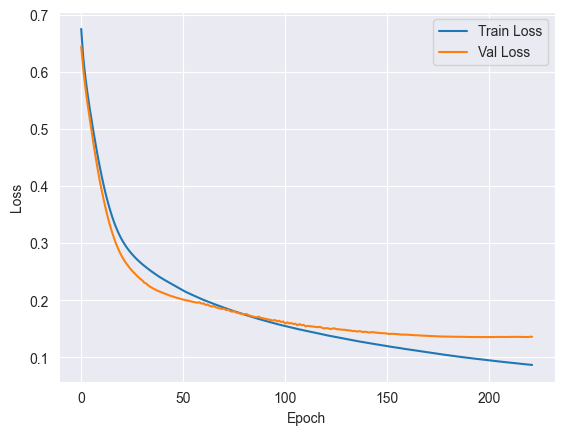
\includegraphics{best.png}
    \caption{Burada Epoch değerini 2000 aldım ve learning rate 0.001. Burada 222. epoch'ta early stopping sayesinde duruyor }
    \label{fig:my_pic}
\end{figure}

% Figure aşağıda comment içindeki kısımdaki gibi eklenir.
\begin{comment}
\begin{figure}[ht!]
    \centering
    \includegraphics[width=0.75\textwidth]{mypicturehere.png}
    \caption{Buraya açıklama yazın}
    \label{fig:my_pic}
\end{figure}
\end{comment}

\pagebreak

\subsection{(10 Puan)} \textbf{SEED=öğrenci numaranız set ettikten sonra altıncı haftada ödev olarak verdiğim gibi earlystopping'deki en iyi modeli kullanarak, Prensesi İyileştir test setinden accuracy, F1, precision ve recall değerlerini hesaplayan kodu yazın ve sonucu da aşağı yapıştırın. \%80'den fazla başarı bekliyorum test setinden. Daha düşükse başarı oranınız, nerede hata yaptığınızı bulmaya çalışın. \%90'dan fazla başarı almak mümkün (ben denedim).}

\begin{python}
from sklearn.metrics import accuracy_score, f1_score, precision_score, recall_score

model.load_state_dict(torch.load('best_model.pt'))

test_predictions = []
test_labels = []
model.eval()
with torch.no_grad():
    for inputs, labels in test_dataloader:
        outputs = model(inputs)
        predicted = torch.round(outputs)
        test_predictions.extend(predicted.detach().cpu().numpy())
        test_labels.extend(labels.detach().cpu().numpy())

accuracy = accuracy_score(test_labels, test_predictions)
f1 = f1_score(test_labels, test_predictions)
precision = precision_score(test_labels, test_predictions)
recall = recall_score(test_labels, test_predictions)

print(f'Accuracy: {accuracy:.4f}')
print(f'F1 score: {f1:.4f}')
print(f'Precision: {precision:.4f}')
print(f'Recall: {recall:.4f}')
\end{python}

Accuracy: 0.9443
F1 score: 0.9436
Precision: 0.9600
Recall: 0.9278

\subsection{(5 Puan)} \textbf{Tüm kodların CPU'da çalışması ne kadar sürüyor hesaplayın. Sonra to device yöntemini kullanarak modeli ve verileri GPU'ya atıp kodu bir de böyle çalıştırın ve ne kadar sürdüğünü hesaplayın. Süreleri aşağıdaki tabloya koyun. GPU için Google Colab ya da Kaggle'ı kullanabilirsiniz, iki ortam da her hafta saatlerce GPU hakkı veriyor.}

\begin{table}[ht!]
    \centering
    \caption{Ben projeyi local bilgisayarımda yaptım bu yüzden sonuçlar biraz ilginç çıktı}
    \begin{tabular}{c|c}
        Ortam & Süre (saniye) \\\hline
        CPU & 12sn \\
        GPU & 28sn\\
    \end{tabular}
    \label{tab:my_table}
\end{table}

\subsection{(3 Puan)} \textbf{Modelin eğitim setine overfit etmesi için elinizden geldiği kadar kodu gereken şekilde değiştirin, validasyon loss'unun açıkça yükselmeye başladığı, training ve validation loss'ları içeren figürü aşağı koyun ve overfit için yaptığınız değişiklikleri aşağı yazın. Overfit, tam bir çanak gibi olmalı ve yükselmeli. Ona göre parametrelerle oynayın.}

Early stopping özelliğini kaldırdım böylece grafik epoch arttıkça overfit etmeye başladı.

\begin{figure}[ht!]
    \centering
    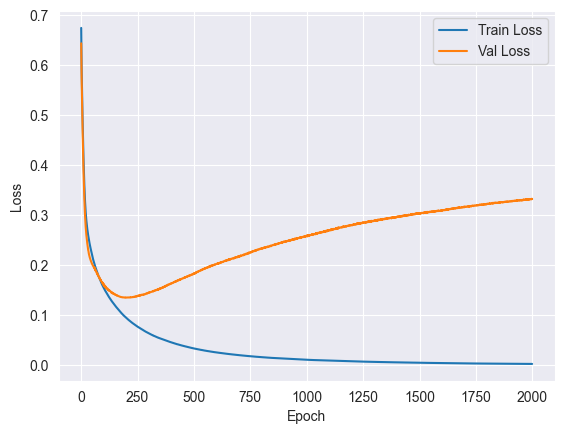
\includegraphics{worst.png}
    \caption{}
    \label{fig:my_psic}
\end{figure}
    

% Figür aşağı
\begin{comment}
\begin{figure}[ht!]
    \centering
    \includegraphics[width=0.75\textwidth]{mypicturehere.png}
    \caption{Buraya açıklama yazın}
    \label{fig:my_pic}
\end{figure}
\end{comment}

\subsection{(2 Puan)} \textbf{Beşinci soruya ait tüm kodların ve cevapların olduğu jupyter notebook'un Github linkini aşağıdaki url'e koyun.}

\url{https://github.com/orypersec/yapay-sinir-aglari-2023/blob/master/soru-5.ipynb}

\section{(Toplam 10 Puan)} \textbf{Bir önceki sorudaki Prensesi İyileştir problemindeki yapay sinir ağınıza seçtiğiniz herhangi iki farklı regülarizasyon yöntemi ekleyin ve aşağıdaki soruları cevaplayın.} 

\subsection{(2 puan)} \textbf{Kodlarda regülarizasyon eklediğiniz kısımları aşağı koyun:} 

\begin{python}
import torch.nn as nn

torch.manual_seed(190401055)

class MLP(nn.Module):
    def __init__(self):
        super(MLP, self).__init__()
        self.hidden_layer_1 = nn.Linear(13, 100)
        self.hidden_layer_2 = nn.Linear(100, 50)
        self.output_layer = nn.Linear(50, 1)
        self.relu = nn.ReLU()
        self.sigmoid = nn.Sigmoid()
        self.dropout = nn.Dropout(0.5)

    def forward(self, x):
        x = self.relu(self.hidden_layer_1(x))
        x = self.dropout(x)
        x = self.relu(self.hidden_layer_2(x))
        x = self.dropout(x)
        x = self.sigmoid(self.output_layer(x))
        return x

model = MLP().to(device)
criterion = nn.BCELoss()
optimizer = torch.optim.SGD(model.parameters(), lr=0.001, weight_decay=0.01)

print(devam_ise_buraya)
\end{python}

\subsection{(2 puan)} \textbf{Test setinden yeni accuracy, F1, precision ve recall değerlerini hesaplayıp aşağı koyun:}

Accuracy: 0.9598
F1 score: 0.9594
Precision: 0.9760
Recall: 0.9433

\subsection{(5 puan)} \textbf{Regülarizasyon yöntemi seçimlerinizin sebeplerini ve sonuçlara etkisini yorumlayın:}

Burada Dropout ve L2 regularizasyonunu seçtim çünkü bu 2 yöntemde overfitting'i engellemek için çok yaygın olarak kullanılan yöntemler bende bu 2 yöntem genelde iyi sonuç verdiği seçtim.

Sonuçların hepsinde ortalama 0.01'lik bir artış oldu ve modelimiz iyileşmiş oldu. Grafikte de zaten açık bir şekilde daha yavaş bir şekilde overfitting olduğu görünüyor.

\subsection{(1 puan)} \textbf{Sonucun github linkini  aşağıya koyun:}

\url{https://github.com/orypersec/yapay-sinir-aglari-2023/blob/master/soru-6.ipynb}

\end{document}